\documentclass[12pt]{beamer}

% INCLUDE GRAPHICS
\usepackage{graphicx}

% TABLES
\newcommand{\ra}[1]{\renewcommand{\arraystretch}{#1}} % spaces in tables
\usepackage{booktabs}   % Allows the use of \toprule, \midrule and \bottomrule in tables for horizontal lines

% FONTS
% PdfLatex
% \usepackage[T1]{fontenc}
% \usepackage{pgf}
% \logo{\pgfputat{\pgfxy(-1,-0.435)}{\pgfbox[center,base]{
\includegraphics[width=1.2cm,natwidth=610,natheight=642]{KUNATLogo.pdf}}}}

% FONTS
% xelatex
\usepackage{fontspec}
% \fontspec[Path=../fonts/,]{
%     UprightFont = *-regular,
%     ItalicFont = *-italic,
%     Boldfont = *-bold
% }

% NOTE
% Add fonts to ~/.fonts for this to work
% \setsansfont{TeX Gyre Heros}
% \setsansfont{TeX Gyre Heros Cn}
% \setsansfont{Liberation Sans}
% \setsansfont{Muli}
% \setsansfont{Helvetica Neue}
\setsansfont{Fira Sans Light}

% Monospaces font
%\setmonofont{Monaco}
\setmonofont{Fira Mono}

% Use serif for Math environments
\usefonttheme[onlymath]{serif}

% CODE
\usepackage{listings} % Code block (source code) \begin{lstlisting}
\lstset{
    language=Python,                        % Code langugage
    commentstyle=\color{gray},              % Comments font
    basicstyle=\scriptsize\ttfamily,             % Code font, Examples: \footnotesize, \ttfamily
    keywordstyle=\bfseries\color{blue},
    stringstyle=\color{orange},
    numbers=left,                           % Line nums position
    numberstyle=\tiny,                      % Line-numbers fonts
    stepnumber=1,                           % Step between two line-numbers
    numbersep=5pt,                          % How far are line-numbers from code
    numbers=none,
    frame=lines,                             % A frame around the code
    rulecolor=\color{gray},
    tabsize=4,                              % Default tab size
    captionpos=b,                           % Caption-position = bottom
    breaklines=true,                        % Automatic line breaking?
    breakatwhitespace=false,                % Automatic breaks only at whitespace?
    showspaces=false,                       % Dont make spaces visible
    showstringspaces=false,                 % Dont make spaces visible in strings
    showtabs=false,                         % Dont make tabls visible
    belowskip=5pt,
    morekeywords={range, xrange},
    backgroundcolor=\color{white}
    % emph={[2]root,base}
    % morekeywords={one,two,three,four,five,six,seven,eight,
}

\newcommand{\code}[1]{{\small\ttfamily #1}} % \code{inline code}

%
% COLORS
%
\definecolor{kugreen}{RGB}{75,116,60}

\definecolor{orange}{RGB}{255,127,0}
\definecolor{green}{RGB}{0,153,51}
\definecolor{blue}{RGB}{3,115,187}
\definecolor{red}{RGB}{221,17,68}
\definecolor{gray}{RGB}{55,55,55}
\definecolor{black}{RGB}{0,0,0}

\definecolor{offwhite}{RGB}{249,242,215}
\definecolor{foreground}{RGB}{23,23,23}
\definecolor{background}{RGB}{255,255,255}
\definecolor{subtitle}{RGB}{102,255,204}
\definecolor{hilight}{RGB}{102,255,204}
\definecolor{vhilight}{RGB}{255,111,207}
\definecolor{lolight}{RGB}{155,155,155}


%
% BEAMER STYLE COLORS
%
\setbeamercolor{titlelike}{fg=black}
\setbeamercolor{subtitle}{fg=blue}
\setbeamercolor{institute}{fg=gray}
\setbeamercolor{normal text}{fg=foreground,bg=background}
\setbeamercolor{item}{fg=foreground} % color of bullets
\setbeamercolor{subitem}{fg=gray}
\setbeamercolor{itemize/enumerate subbody}{fg=gray}

\setbeamerfont{itemize/enumerate subbody}{size=\footnotesize}
\setbeamerfont{itemize/enumerate subitem}{size=\footnotesize}

\setbeamerfont{footnote}{size=\tiny}

\setbeamersize{text margin left=10pt}
\setbeamersize{text margin right=10pt}
\setbeamersize{sidebar width right=0pt}
\setbeamersize{sidebar width left=0pt}

%
% REMOVES THE NAVIGATION BAR
%
\beamertemplatenavigationsymbolsempty


% BEAMER TEMPLATES


%
% BEAMER BACKGROUND
%
\usebackgroundtemplate{

    \rule{0pt}{0.985\paperheight}% down
    \hspace*{1.41\paperwidth}% right
    \makebox[0pt][r]{%
        
\includegraphics[width=200pt,natwidth=610,natheight=642]{images/KUNATLogo_2016.pdf}
    }

}


%
% BEAMER HEADLINE
%
\setbeamertemplate{headline}{}


%
% BEAMER TITLE
%
\setbeamertemplate{frametitle}
{
    \begin{centering}
    \insertframetitle\par
    \end{centering}
}


%
% BEAMER FOOTER
%
\setbeamertemplate{footline}[text line]
{%
    \vbox{%
        \insertvrule{0.5pt}{kugreen}

        \vspace{2pt}

        \strut{
        % \rmfamily\itshape
        \expandafter\insertshorttitle
        \expandafter\insertauthor
        \insertshortinstitute
        }
        \hfill\strut{
        }
        \hfill\strut{
            \insertframenumber\,/\,\inserttotalframenumber
        }

        \vspace{1pt}
    }
}


%
% TITLE PAGE
%
% \setbeamertemplate{title page}
% {
%     % Remove beamer background
%     \setbeamertemplate{background}{}
% 
%     \begin{beamercolorbox}[center]{beamer color}
% 
%         {
%             \huge
%             \color{kugreen}
%             \inserttitle
%         }
%         \bigskip
%         \bigskip
% 
%         % 
\includegraphics[width=2cm]{KUNATLogo}
% 
%         \bigskip
%         {
%             \bf
%             \rmfamily
%             {\large \insertauthor}
%         }
% 
%         \smallskip
%         {
%             \rmfamily
%             \footnotesize
%             \insertinstitute
%         }
% 
%         {
%             \rmfamily
%             \footnotesize
%             \insertdate
%         }
% 
%     \end{beamercolorbox}
% 
%     % Do not count the title page
%     \addtocounter{framenumber}{-1}
% }


% MACRO
\renewcommand{\sup}[1]{$^\text{#1}$}
\newcommand{\sub}[1]{$_\text{#1}$}
\newcommand{\set}     [1] {\{#1\}}


\usepackage{soul}

\title[]{So... what do you do for a living?}


\institute[, University of Copenhagen]{Department of Chemistry \\ University of Copenhagen}

\author[J. C. Kromann]{Jimmy Charnley Kromann \newline PhD Student $\in$ Jan Jensen Group}

\date{
    \code{\scriptsize jimmy@charnley.dk}
}




% ===============
% begin slides
% ===============


\begin{document}

{
\usebackgroundtemplate{}
\begin{frame}[plain]
    \titlepage
    \addtocounter{framenumber}{-1}
\end{frame}
}

{

\usebackgroundtemplate{

    \rule{0pt}{1.35\paperheight}%
    \hspace*{1.15\paperwidth}%
    \makebox[-4pt][r]{%
        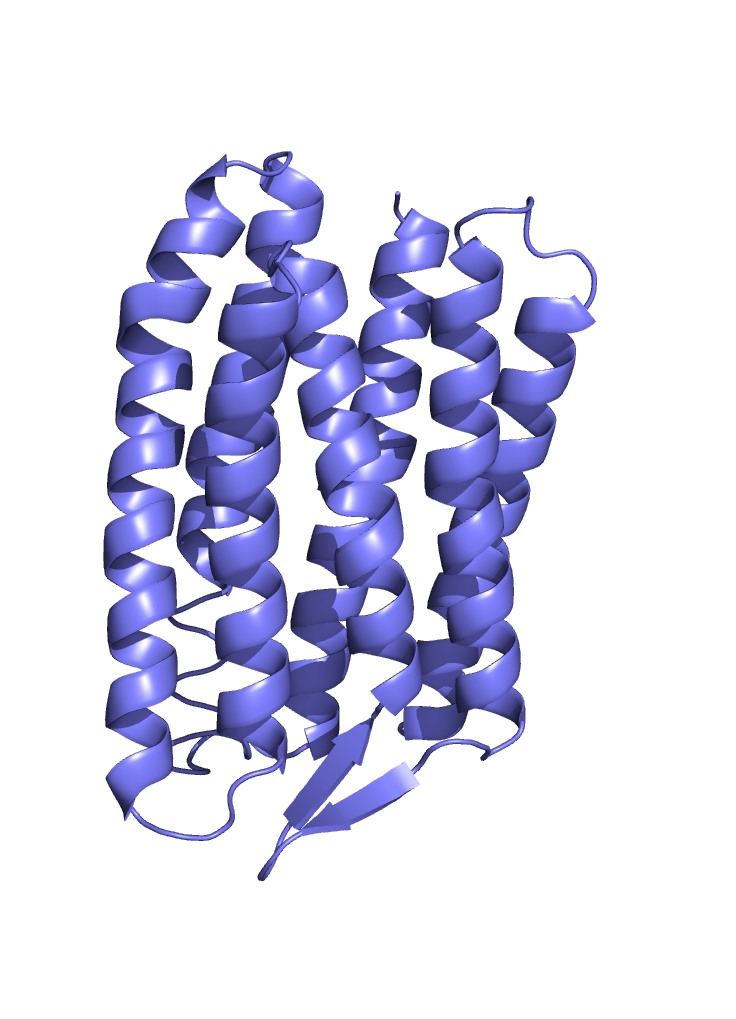
\includegraphics[width=220pt]{images/1h68.png}%
    }

}

\begin{frame}[fragile]

    \frametitle{Motivational speech}

    Development of Methods for Computational Bio-chemistry Problems,
    such as;

    \bigskip

    \begin{columns}[c]
        \column{0.7\linewidth}

    \begin{itemize}
        \item Protein Structure determination
        \item Predicting and designing enzyme reactions
        \item Predicting and designing drugs \newpage
            {\scriptsize (host - ligand binding, pKa Values) }
    \end{itemize}

        \column{0.3\linewidth}
    \end{columns}

\end{frame}
}



\begin{frame}[fragile]

    \frametitle{Methodology available}

    \begin{columns}[t]
        \column{0.33\linewidth}
        \centering
        Force Fields
        \column{0.33\linewidth}
        \centering
        {\bf Semi-empirical}
        \column{0.33\linewidth}
        \centering
        Fragmentation
    \end{columns}

    \bigskip
    \bigskip

{
    \scriptsize

    \begin{tabular*}{\linewidth}{ @{} l l l l @{} }
        Name & Author & Ref & DOI \\
        \midrule
        {\bf PM6} & Stewart            & J Mol Model {\bf 2007} 13:1173 & 10.1007/s00894-007-0233-4 \\
     {\bf DFT-D3} & Grimme {et al}     & J Chem Phys {\bf 2010} 15:154104 & 10.1063/1.3382344 \\
    {\bf PM6-DH+} & Korth              & J Chem T Comp {\bf 2010} 12:3808 & 10.1021/ct100408b \\
    {\bf PM6-D3H} & Grimme             & Chem Eur J  {\bf 2012} 18:9955 & 10.1002/chem.201200497 \\
      {\bf HF-3c} & Sure \& Grimme     & J Comput Chem {\bf 2013} 19:1672 &  10.1002/jcc.23317 \\

    \end{tabular*}
}
    \small

    \bigskip

    Most use PM6 $\in$ MOPAC

    \bigskip

    HF-3c: HF/minimal basis set corrected for dispersion \& BSSE using 9 parameters. {\em No experimental input. }

\end{frame}


\begin{frame}[fragile]
    \frametitle{Importance of optimizers}

    \begin{center}
        in free energy calculations

    \end{center}

    \begin{columns}[t]
        \column{0.5\linewidth}

        \centering

        \begin{tabular}{@{} l r r r @{} }

            [kcal/mol] & $\Delta H_f$ & $-T\Delta S$ & $N_i$ \\

          \midrule

          1 & -523.75 & -108.18 & 21 \\
          2 & -521.19 & -102.25 & 4 \\
          3 & -523.12 & -101.34 & 4 \\
          4 & -521.28 & -102.40 & 4 \\
          5 & -522.73 & -102.15 & 6 \\
          6 & -521.52 & -103.26 & 7 \\
          7 & -521.85 & -102.86 & 7 \\

          \midrule

          $\Delta$ & 2.56 & 6.84

        \end{tabular}

        \column{0.5\linewidth}

        \centering
 
        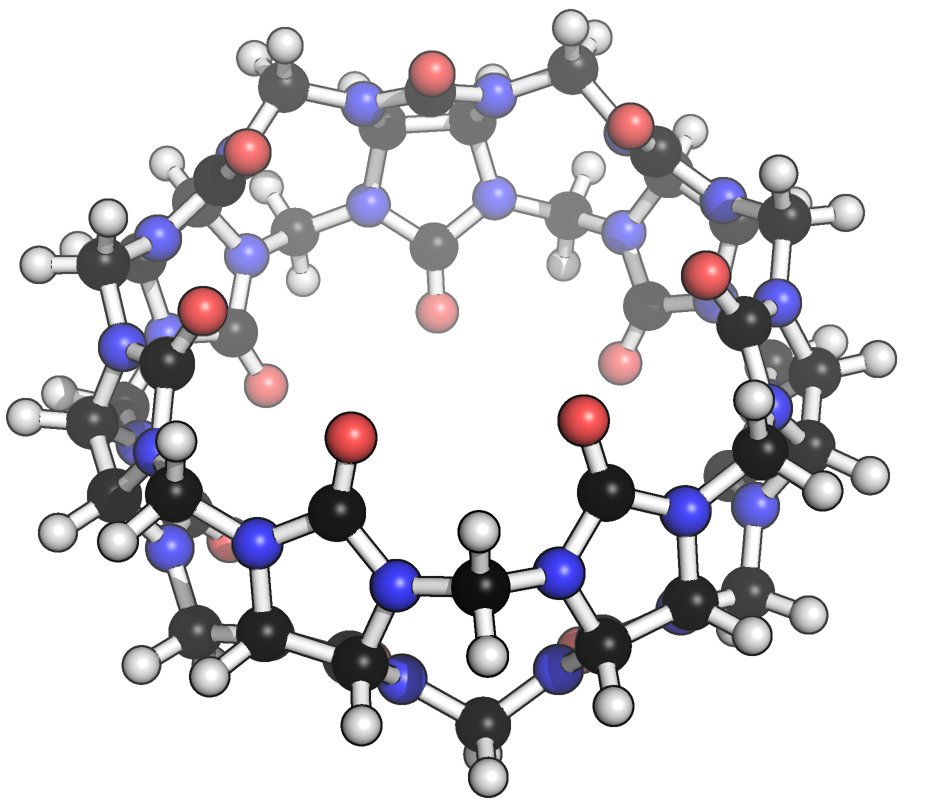
\includegraphics[width=0.9\linewidth]{images/cb7-a.png}

        \bigskip

    \end{columns}

    \bigskip

    \small
    Small conformational changes in start structure,\newline using PM6-DH+/COSMO $\in$ MOPAC


\end{frame}


\begin{frame}[fragile]

    \frametitle{Good Artists Copy; Great Artists Steal}

    \centering
    and puts the source code in GAMESS

    \begin{align*}
        { \overbrace{E(\mathrm{PM6\text{-}D3H+})}^\text{Kromann et al} } =
        { \overbrace{ E(\mathrm{PM6}) }^\text{Stewart} } +
        { \overbrace{ E(\mathrm{D3}) }^\text{Grimme et al} } +
        { \overbrace{ E(\mathrm{H+}) }^\text{Korth} }
    \end{align*}

    \bigskip

    {\scriptsize
        {\bf J. C. Kromann}, A. S. Christensen, C. Steinmann, M. Korth and J. H. Jensen\\
        PeerJ
        {\bf 2014}
        2:e449
        {10.7717/peerj.449}
    }

    \bigskip

    \bigskip

    \bigskip

    Interface of HF-3c/Fragment Molecular Orbitals

    \bigskip

    {\scriptsize
        {\bf J. C. Kromann} and J. H. Jensen\\
        Unpublished (Need to fix a basis set error for very-heavy atoms)
    }

\end{frame}


\begin{frame}[fragile]
    \frametitle{Interaction energies}
    \centering 

    \bigskip

    \begin{minipage}[t]{0.65\textwidth}
            {

            \scriptsize

            \begin{tabular}{ @{} l r r r r @{} }
                \ra{1.3}
                [kcal/mol]
                & {\color{red}PM6}
                & {\color{blue}PM6-DH+}
                & {\color{kugreen}PM6-D3H+}
                & HF-3c \\
                \midrule
                \multicolumn{5}{c}{\small All Complexes} \\
                \midrule

                RMSD & {\color{red}3.35} & {\color{blue}0.80} & {\color{kugreen}0.82} & {0.54} \\
                 MAD & {\color{red}2.85} & {\color{blue}0.61} & {\color{kugreen}0.60} & {1.80} \\

                 Max & {\color{red}7.99} & {\color{blue}2.47} & {\color{kugreen}2.11} & {1.80} \\

                && \\
                \multicolumn{5}{c}{ \small Dispersion Complexes} \\
                \midrule

                RMSD & {\color{red}3.15} & {\color{blue}0.49} & {\color{kugreen}0.48} & {0.63} \\
                 MAD & {\color{red}2.79} & {\color{blue}0.42} & {\color{kugreen}0.36} & {1.80} \\

                 Max & {\color{red}7.99} & {\color{blue}2.47} & {\color{kugreen}2.11} & {1.80} \\

                && \\
                \multicolumn{5}{c}{ \small Hydrogen-bond Complexes} \\
                \midrule

                RMSD & {\color{red}4.29} & {\color{blue}0.98} & {\color{kugreen}1.11} & {0.58} \\
                 MAD & {\color{red}3.65} & {\color{blue}0.80} & {\color{kugreen}0.92} & {1.36} \\
                 Max & {\color{red}7.99} & {\color{blue}2.10} & {\color{kugreen}1.85} & {1.36} \\

            \end{tabular}

            }

    \end{minipage}
    \begin{minipage}[c]{0.33\textwidth}

            \centering

            {
                begdb.com

                S22 \& S66
            }
    
            \bigskip

            {

            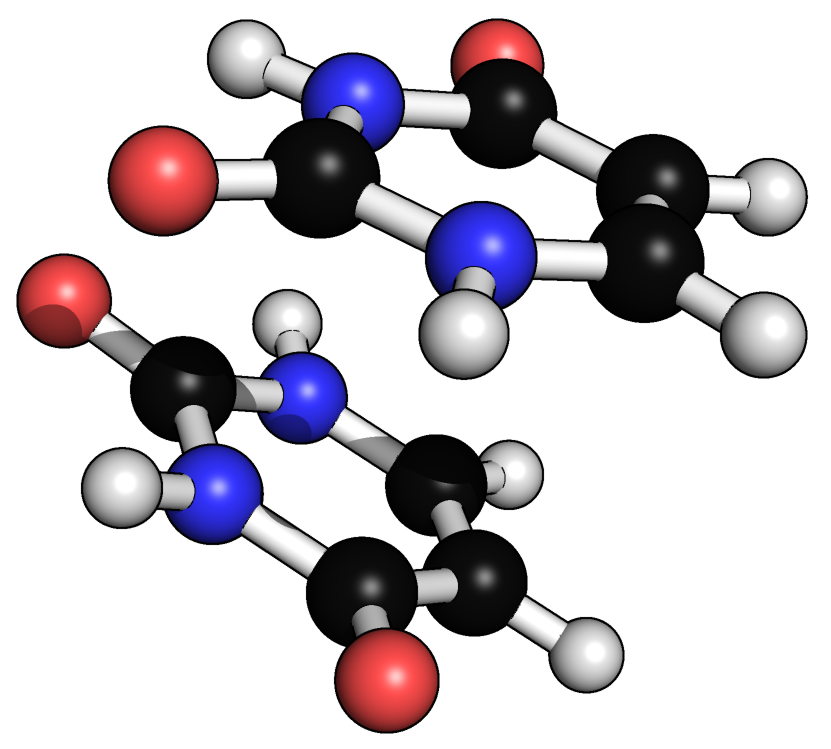
\includegraphics[width=1.0\linewidth]{images/s22_13.png}
 
            }

    \end{minipage}
\end{frame}

\begin{frame}[fragile]
    \frametitle{Optimize S22 \& S66}

    \centering

    {\scriptsize

    \begin{tabular}{@{} l r r r r r @{} }
        & avg. RMSD [\AA]
        & HB RMSD [\AA]
        & $\bar {N_S}$
        & avg. Gnorm
        & $\bar N_i$ (max)\\
        \midrule
        
        && \\
        \multicolumn{6}{c}{ MOPAC } \\
        \midrule

        %MOPAC
        PM6        &  0.28 & 0.24 & 229 & 1.4$\cdot$10\sup{-3} &  0.71 (6) \\
        PM6-DH+    &  0.21 & 0.24 & 376 & 2.3$\cdot$10\sup{-3} &  0.79 (9) \\

        && \\
        \multicolumn{6}{c}{ GAMESS } \\
        \midrule

        % GAMESS
        PM6          &  0.11 & 0.13 &  30 & 1.0$\cdot$10\sup{-4} &  0.02 (1) \\
        PM6-D3H+     &  0.12 & 0.08 &  31 & 1.0$\cdot$10\sup{-4} &  0.07 (1) \\
         HF-3c     &  0.10 & 0.05 & 32 & 1.1$\cdot$10\sup{-4} &  0.51 (3) \\

    \end{tabular}

    }

    \bigskip

    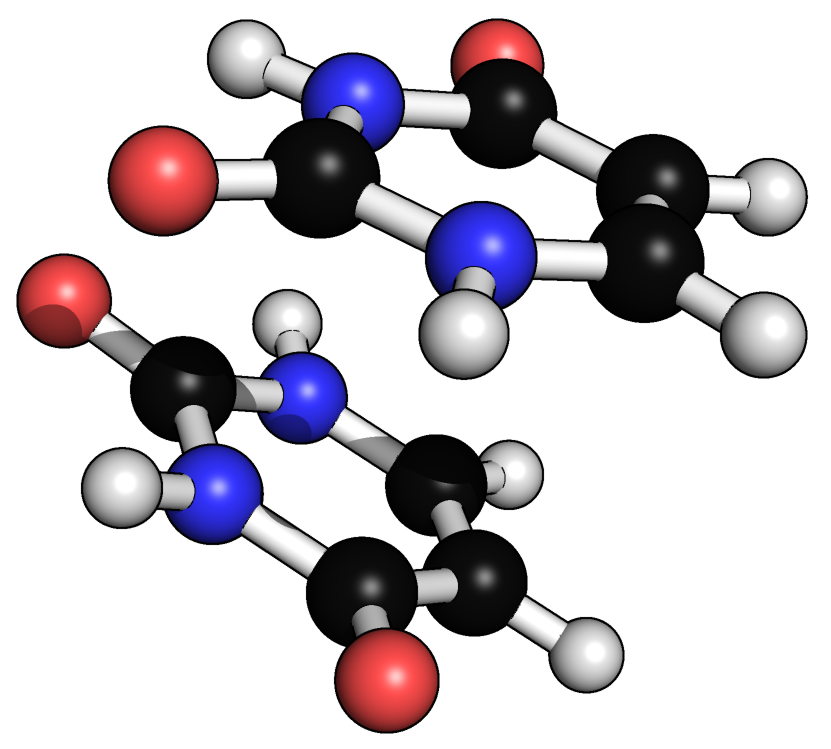
\includegraphics[width=0.2\linewidth]{images/s22_13.png}

\end{frame}

\begin{frame}[fragile]
    \frametitle{Same example as earlier}

    \begin{columns}[t]
        \column{0.5\linewidth}

        \centering

        \begin{tabular}{@{} l r r r @{} }

            [kcal/mol] & $\Delta H_f$ & $-T\Delta S$ & $N_i$ \\

          \midrule

          1 & -513.91 & -99.50 & 0 \\
          2 & -512.74 & -100.68 & 0 \\
          3 & -512.96 & -101.33 & 0 \\
          4 & -512.98 & -101.23 & 0 \\
          5 & -514.30 & -100.07 & 0 \\
          6 & -514.26 & -100.34 & 0 \\
          7 & -512.63 & -100.67 & 0 \\

          \midrule

          $\Delta$ & 1.67 & 1.83 

          % $\Delta$ & 2.56 & 6.84 before

        \end{tabular}

        \column{0.5\linewidth}

        \centering

        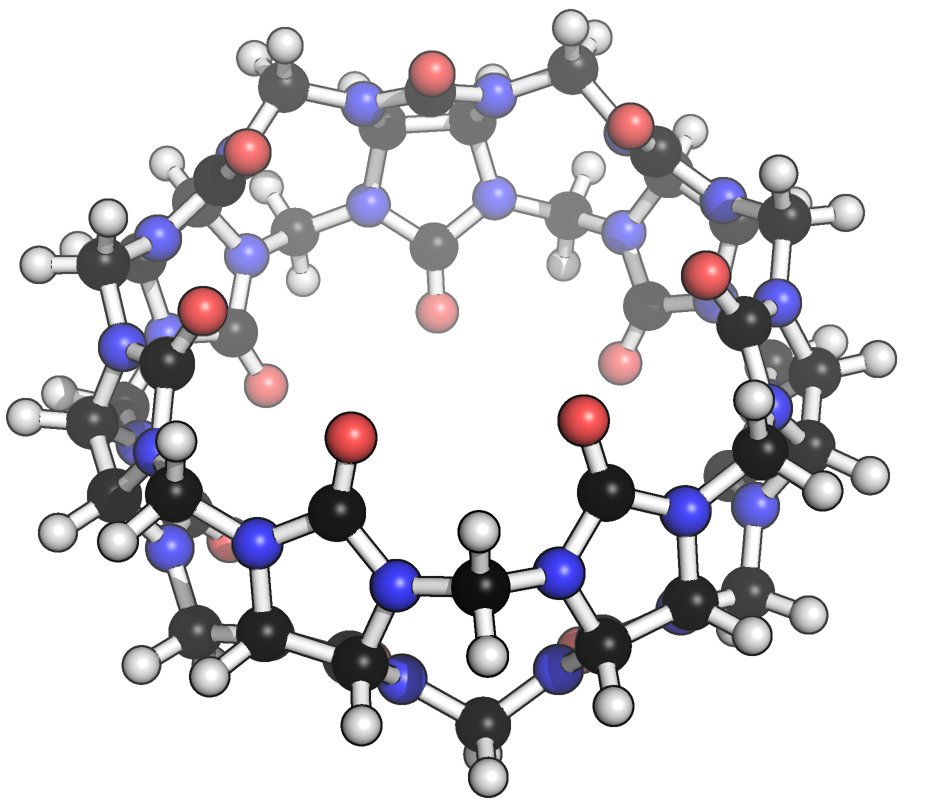
\includegraphics[width=0.9\linewidth]{images/cb7-a.png}

    \end{columns}

    \bigskip
    \small
    Small conformational changes in start structure,\newline using PM6-D3H+/PCM $\in$ GAMESS

\end{frame}


\begin{frame}[fragile]
    \frametitle{What about pKa prediction?}

    \begin{equation*}
    \mathrm{pK_a}=\mathrm{pK_a^{ref}} + \frac{\Delta G^\circ}{RT\ln (10)} 
    \end{equation*}

    \bigskip

    Reference DFT Calculations\newline
    {\bf Sastre et al. 2012.}\newline doi: 10.1007/s00214-012-1310-z

    \bigskip

    {\bf Jensen.} 2015. High Througput pKa Prediction Using Semi Empirical Methods. arXiv:1512.00701

    \bigskip

    {\bf Kromann et al.}\newline doi: 10.7287/peerj.preprints.2075v1 (submitted)


% \caption{Mean absolute differences (MADs) and maximum absolute difference (Max AD) of predicted pKa values relative to experimental values for the molecules listed in Table \ref{tab:molecules}. 
% CBS-4B3*, B3LYP, and M05-2X refer to predictions made by \citet{Sastre_2012} using a modified CBS-4B3 composite method and the SMD solvation method, B3LYP/6-311++G(d,p)/SMD and M05-2X/6-311++G(d,p)/SMD, respectively. 
% The "**" indicates MAD and Max AD computed for primary amines only. The "*" indicates that the rigid rotor, harmonic oscillator free energy term is neglected.}
%\textbf{The "**" indicates MAD and Max AD computed for primary amines only. The "*" indicates that the rigid rotor, harmonic oscillator free energy term is neglected.}}

\end{frame}


\begin{frame}[fragile]
    \frametitle{pKa}

    \scriptsize
\begin{table}[htb]
\begin{tabular}{lccccccc}
\midrule
                  & B3LYP/& PM6-D3H+/ & PM6-D3H+/ & PM6/ & PM6/ \\
                  & SMD   & SMD       & SMD*      & SMD* & COSMO* \\
\midrule
\textbf{Amines}  &       &          &          &         &           \\
MAD              & 0.4   & 1.2      & 1.2      & 1.3     & 0.7       \\
Max AD           & 0.8   & 3.9      & 4.0      & 4.1     & 1.9       \\
MAD**            & 0.4   & 0.5      & 0.6      & 0.6     & 0.6       \\
Max AD**         & 0.8   & 1.2      & 1.4      & 1.4     & 1.4       \\
\textbf{Carboxylic acids}\\
MAD              & 0.7   & 1.4      & 1.3      & 1.2     & 1.0       \\
Max AD           & 1.5   & 3.5      & 3.3      & 3.3     & 2.3       \\
\textbf{Pyuidines}\\
MAD              & 0.6   & 0.2      & 0.3      & 0.3     & 0.4       \\
Max AD           & 1.0   & 0.4      & 0.4      & 0.5     & 1.0       \\
\textbf{Alcohols}\\
MAD              & 1.0   & 0.7      & 0.8      & 0.8     & 0.8       \\
Max AD           & 2.3   & 1.7      & 1.9      & 1.8     & 1.9       \\
\textbf{Phenols}\\
MAD              & 0.9   & 1.3      & 1.2      & 1.2     & 1.3       \\
Max AD           & 2.2   & 2.4      & 2.5      & 2.4     & 2.4       \\
\textbf{Benzoic Acids}\\
MAD              & 0.5   & 0.3      & 0.3      & 0.3     & 0.3       \\
Max AD           & 1.4   & 0.7      & 0.7      & 0.7     & 0.7  \\
\midrule
\end{tabular}
\end{table}




\end{frame}



\begin{frame}[fragile]
    \frametitle{What about enzymes barriers}
    


    \begin{center}

        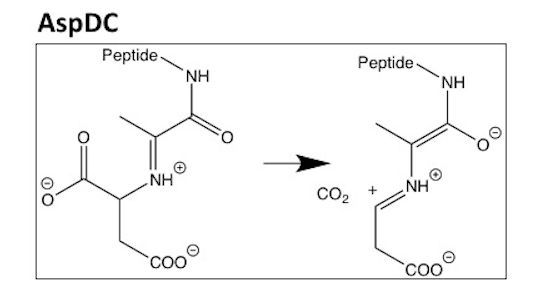
\includegraphics[width=0.5\linewidth]{images/enzymes.png}

        \small

        Towards a barrier height benchmark set
    
        for biologically relevant systems

    \end{center}

    \bigskip

    \centering

    Kromann, Christensen, Cui, Jensen (2016) PeerJ.
    
    doi: 10.7717/peerj.1994


\end{frame}

\begin{frame}[fragile]
    \frametitle{What about enzymes barriers}

    \bigskip

    \small

    \begin{itemize}
        \item All structures available at github.com/jensengroup/db-enzymes
        \item All reference at B3LYP/6-311+G(2d,2p)//B3LYP/6-31G(d,p)
        \item The MADs for PM6 and PM7 was 10-15 kcal/mol
        \item The MADs for DFTB was 6 kcal/mol
    \end{itemize}

    \begin{itemize}
        \item We need better references
        \item We need more references
    \end{itemize}

\end{frame}


\begin{frame}[fragile]

    \frametitle{Okay, and what are you working on now?}

    \begin{itemize}
        \item $d$-orbitals missing for PM6 in GAMESS
    \end{itemize}

    \bigskip

    \begin{itemize}
        \item "name to pKa" predictor
    \end{itemize}

    \bigskip

    \begin{itemize}
        \item More work on enzymes
    \end{itemize}

\end{frame}


\begin{frame}[fragile]
    \frametitle{Shameless self-promotion}

    % TODO KU billede

    \begin{columns}[t]
        \column{0.5\linewidth}
        
        \footnotesize

        {\bf Jensen Group}

        proteinsandwavefunctions.blogspot.com

        github.com/jensengroup

        \bigskip

        {\bf Jimmy stuff}

        computerandchemistry.blogspot.com

        github.com/charnley
        
        {\scriptsize (Please use my code)}

        \column{0.5\linewidth}

        \centering
        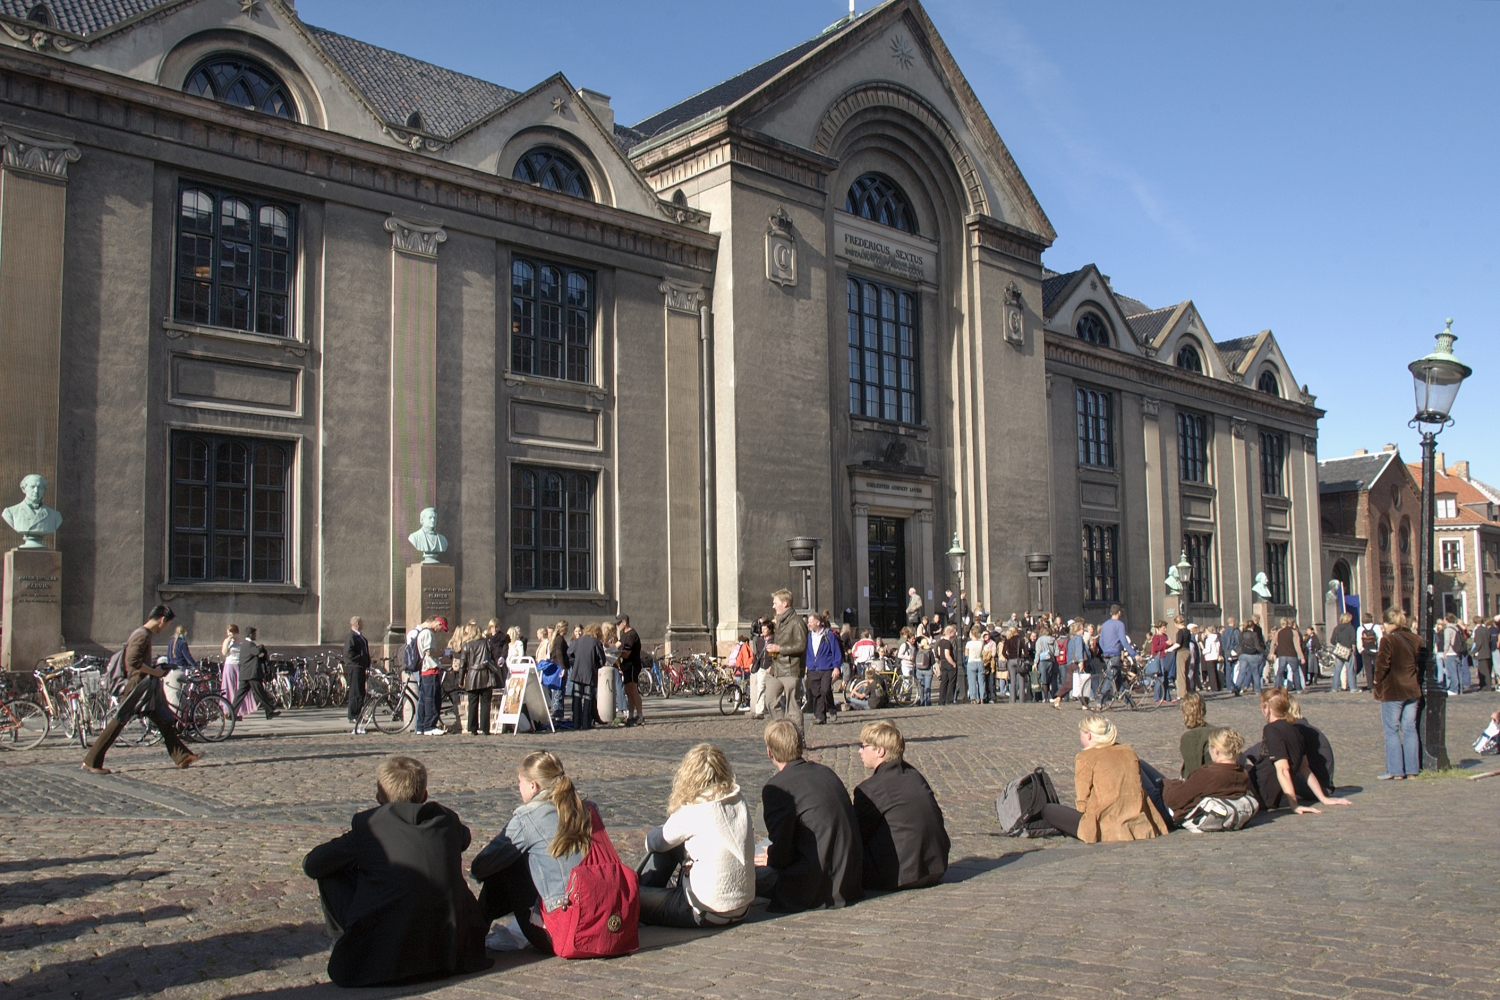
\includegraphics[width=0.9\linewidth]{images/ku.jpg}

    \end{columns}

\end{frame}

% APPENDIX

\usebackgroundtemplate{}

\begin{frame}[fragile]
    \addtocounter{framenumber}{-1}
    \frametitle{}
\end{frame}

\begin{frame}[fragile]
    \addtocounter{framenumber}{-1}
    \frametitle{pKa Calculation}

    \begin{equation}
    \mathrm{pK_a}=\mathrm{pK_a^{ref}} + \frac{\Delta G^\circ}{RT\ln (10)} 
    \end{equation}

    \bigskip

    \begin{equation}
    \mathrm{ BH^+ + B_{ref} \rightleftharpoons B + B_{ref}H^+ }
    \end{equation}

    \bigskip

    \begin{equation}
    \label{eqn:deltag}
    G^\circ(X) = \Delta H_f(X) + [G^\circ_{RRHO}(X)]+\Delta G^\circ_{solv}(X)
    \end{equation}

\end{frame}


%%%%%%%%%%%%%%%%%%%%%%%%%%%%%%%%%%%%%%%%%%%%%%%%%%%%%%%%%%%%%%%%%%%%%%
%% END FRAMES
%%%%%%%%%%%%%%%%%%%%%%%%%%%%%%%%%%%%%%%%%%%%%%%%%%%%%%%%%%%%%%%%%%%%%%

\end{document}

